%%%%%%%%%%%%%%%%%%%%%%%%%%%%%%%%%%%%%%%%%
% Beamer Presentation
% LaTeX Template
% Version 1.0 (10/11/12)
%
% This template has been downloaded from:
% http://www.LaTeXTemplates.com
%
% License:
% CC BY-NC-SA 3.0 (http://creativecommons.org/licenses/by-nc-sa/3.0/)
%
%%%%%%%%%%%%%%%%%%%%%%%%%%%%%%%%%%%%%%%%%
%HOLA
%----------------------------------------------------------------------------------------
%	PACKAGES AND THEMES
%----------------------------------------------------------------------------------------


\documentclass{beamer}

\mode<presentation> {

% The Beamer class comes with a number of default slide themes
% which change the colors and layouts of slides. Below this is a list
% of all the themes, uncomment each in turn to see what they look like.

%\usetheme{default}
%\usetheme{AnnArbor}
%\usetheme{Antibes}
%\usetheme{Bergen}
%\usetheme{Berkeley}
\usetheme{Berlin}
%\usetheme{Boadilla}
%\usetheme{CambridgeUS}
%\usetheme{Copenhagen}
%\usetheme{Darmstadt}
%\usetheme{Dresden}
%\usetheme{Frankfurt}
%\usetheme{Goettingen}
%\usetheme{Hannover}
%\usetheme{Ilmenau}
%\usetheme{JuanLesPins}
%\usetheme{Luebeck}
%\usetheme{Madrid}
%\usetheme{Malmoe}
%\usetheme{Marburg}
%\usetheme{Montpellier}
%\usetheme{PaloAlto}
%\usetheme{Pittsburgh}
%\usetheme{Rochester}
%\usetheme{Singapore}
%\usetheme{Szeged}
%\usetheme{Warsaw}

% As well as themes, the Beamer class has a number of color themes
% for any slide theme. Uncomment each of these in turn to see how it
% changes the colors of your current slide theme.

%\usecolortheme{albatross}
\usecolortheme{beaver}
%\usecolortheme{beetle}
%\usecolortheme{crane}
%\usecolortheme{dolphin}
%\usecolortheme{dove}
%\usecolortheme{fly}
%\usecolortheme{lily}
%\usecolortheme{orchid}
%\usecolortheme{rose}
%\usecolortheme{seagull}
%\usecolortheme{seahorse}
%\usecolortheme{whale}
%\usecolortheme{wolverine}

%\setbeamertemplate{footline} % To remove the footer line in all slides uncomment this line
%\setbeamertemplate{footline}[page number] % To replace the footer line in all slides with a simple slide count uncomment this line

%\setbeamertemplate{navigation symbols}{} % To remove the navigation symbols from the bottom of all slides uncomment this line
}
%BEAVER BERLIN LA MEJOR
\usepackage[spanish.mexico]{babel}
\usepackage[T1]{fontenc}
\usepackage[utf8]{inputenc}



%DIAGRAMAS
\usepackage{smartdiagram}
\usesmartdiagramlibrary{additions}

%Plotting

\usepackage{pgfplots}
\pgfplotsset{width=10cm,compat=1.9} 
%\usepgfplotslibrary{external}
%\tikzexternalize 

%Graficos e imagenes
\usepackage{graphicx}
%\graphicspath{ Imagenes/ }
\usetikzlibrary{arrows}

\usepackage{natbib}
\usepackage{cite}

\usepackage{subcaption}

%Grafico de barras
%\usepackage{pgfplots}


\usepackage{tikz}
\usepackage[american voltages, american currents,siunitx]{circuitikz}

%\usepackage{graphicx} % Allows including images
\usepackage{booktabs} % Allows the use of \toprule, \midrule and \bottomrule in tables

%----------------------------------------------------------------------------------------
%	TITLE PAGE
%----------------------------------------------------------------------------------------

\title[Radiación en seres vivos]{Efectos de la radiación sobre seres Vivos} % The short title appears at the bottom of every slide, the full title is only on the title page




\author{Daniela García Zavala,Pablo Vivar Colina} % Your name
\institute[UNAM] % Your institution as it will appear on the bottom of every slide, may be shorthand to save space
{
Facultad de Ingeniería de la Universidad Nacional Autónoma de México \\ % Your institution for the title page
\medskip
\textit{dani.g.z-95@comunidad.unam.mx\\
pvivar@idea161.org} % Your email address
}
%\date{\today} % Date, can be changed to a custom date
\date{Octubre 2019}

\begin{document}

\begin{frame}
\titlepage % Print the title page as the first slide
\end{frame}

\begin{frame}
\frametitle{Secciones} % Table of contents slide, comment this block out to remove it
\tableofcontents % Throughout your presentation, if you choose to use \section{} and \subsection{} commands, these will automatically be printed on this slide as an overview of your presentation
\end{frame}

%----------------------------------------------------------------------------------------
%	PRESENTATION SLIDES
%----------------------------------------------------------------------------------------

%------------------------------------------------




\section{Biología Elemental}
 % Sections can be created in order to organize your presentation into discrete blocks, all sections and subsections are automatically printed in the table of contents as an overview of the talk
%------------------------------------------------

\begin{frame}
	%\frametitle{}

  \begin{block}{}
	El efecto de la radiación en los seres vivos se debe a la excitación o ionización de varias moléculas contenidas en las células que forman un sistema vivo.\\
  \end{block}

  \begin{block}{}
	Hay aproximadamente $4 x 10^{13}$ células en una persona adulta promedio.
  \end{block}

% Estas, sin embargo, no son todas idénticas, ni en función ni en tamaño. Células cerebrales obviamente realizar una función diferente a las células del hígado. La mayoría de las células son bastante pequeñas, en el orden de 
  \begin{block}{Tamaño de células en promedio}
	$10^{-3}$ [cm] de diámetro
  \end{block}

  \begin{block}{Células nerviosas}
	1 [m] longitud
  \end{block}

%; las células nerviosas, por el contrario, pueden tener un metro de largo.\\	
\end{frame}

%------------------------------------------------

\begin{frame}
	
	\begin{block}{}
	   Las células contienen varias estructuras orgánicas llamadas orgánulos, cada una de las cuales realiza funciones específicas para la célula como lo hacen los órganos en el cuerpo como un todo.\\
	   	
	\end{block}
	
	
	\begin{block}{}
	  Estos orgánulos están suspendidos en el citoplasma, una mezcla diluida transparente de agua y diversas moléculas y electrolitos, que comprende la mayor parte de la célula volumen. Otras partes principales de la celda que se muestran en la figura \ref{celula}  son:\\		
	\end{block}
	
\end{frame}

%------------------------------------------------

\begin{frame}
  \begin{figure}[h!]
  	\centering
  	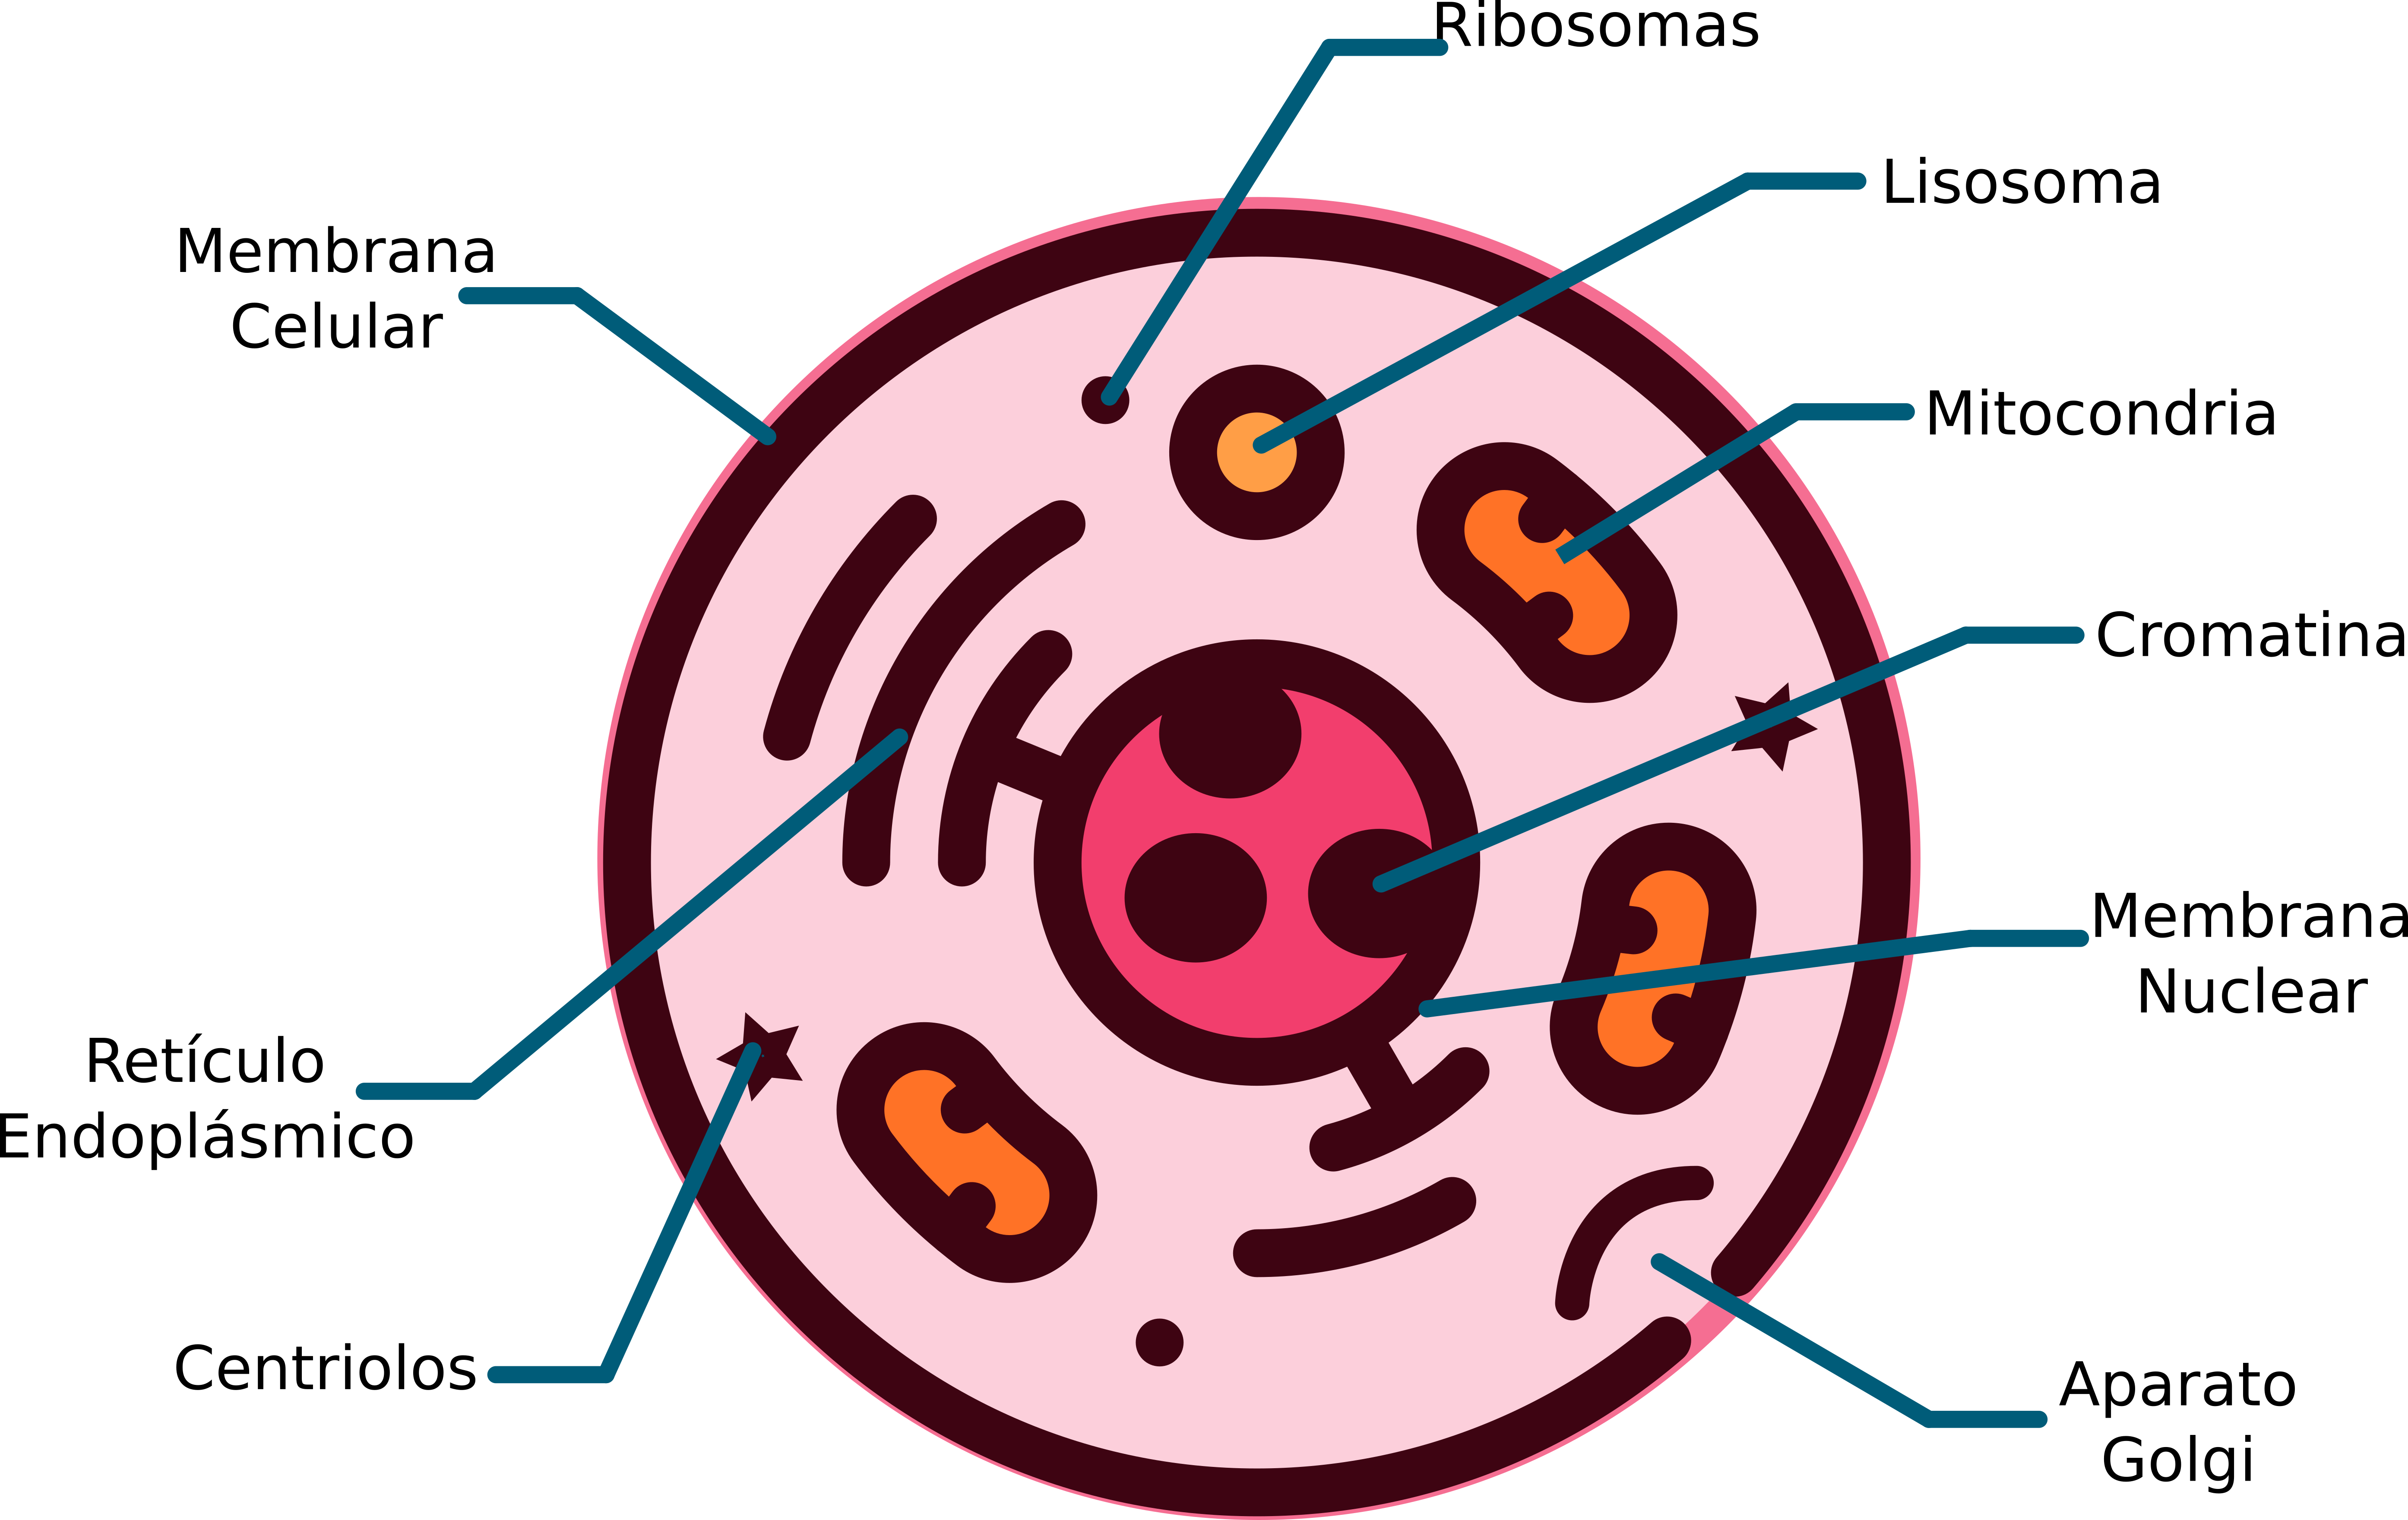
\includegraphics[width=0.6\textwidth]{celula.png}
  	\caption{Célula somática tradicional}
  	\label{celula}
  \end{figure}	
\end{frame}

%------------------------------------------------

\begin{frame}
	\begin{figure}
		\begin{minipage}[t][3.5cm]{\textwidth}
			\begin{center}
				\smartdiagramset{
					%uniform color list=gray!60!black for 3 items,
					back arrow disabled=true,
					additions={
						additional item offset=0.85cm,
						additional item border color=blue,
						%additional arrow color=red,
						%additional arrow tip=stealth,
						%additional arrow line width=1pt,
						%additional arrow style=]-latex’,
					}
				}
				\smartdiagramadd[bubble diagram:horizontal]{Células,Somáticas,Germinales}{%
					%
				}
			\end{center}
		\end{minipage}
		\caption{}
		\label{tiposCelulas}
	\end{figure}	
\end{frame}

%------------------------------------------------

\begin{frame}

  \begin{block}{Núcleo}
	Este es el cuerpo grande, generalmente esférico, que funciona como control central de la célula; Contiene la cromatina.
  \end{block}

  \begin{block}{Cromatina}
	Cromatina Este es el material genético de la célula.
  \end{block}

  \begin{block}{Nucleolo}
	 Estos son cuerpos esféricos (puede haber tantos como cuatro ubicados en el núcleo) que son importantes en el metabolismo de ciertos productos químicos.
  \end{block}

\end{frame}

%------------------------------------------------

\begin{frame}

  \begin{block}{Retículo endoplásmico}
	Esta es una red compleja de túbulos aplanados que sirve para transportar materiales dentro de la célula y es también una fuente importante de enzimas metabólicas.
  \end{block}

  \begin{block}{Aparato de Golgi}
	Las funciones de este orgánulo no se entienden completamente. El Aparato de Golgi aparentemente concentra y modifica ciertas sustancias químicas.
  \end{block}
	
\end{frame}

%------------------------------------------------

\begin{frame}
	
  \begin{block}{Lisosomas y peroxisomas}
	Estos orgánulos contienen enzimas para producir diversos productos químicos.
  \end{block}

  \begin{block}{Centriolos}
	Estos orgánulos ocurren en pares y son esenciales en la división de mitosis o células.
  \end{block}

  \begin{block}{Ribosomas}
	Estos son los centros para la producción de proteínas; Ellos están localizados en el retículo endoplásmico, en la superficie del núcleo y en el citoplasma.
  \end{block}
	
\end{frame}

%------------------------------------------------


 \begin{frame}
 	
       \begin{figure}[h!]
       	\centering
       	\begin{subfigure}[b]{0.45\textwidth}
       		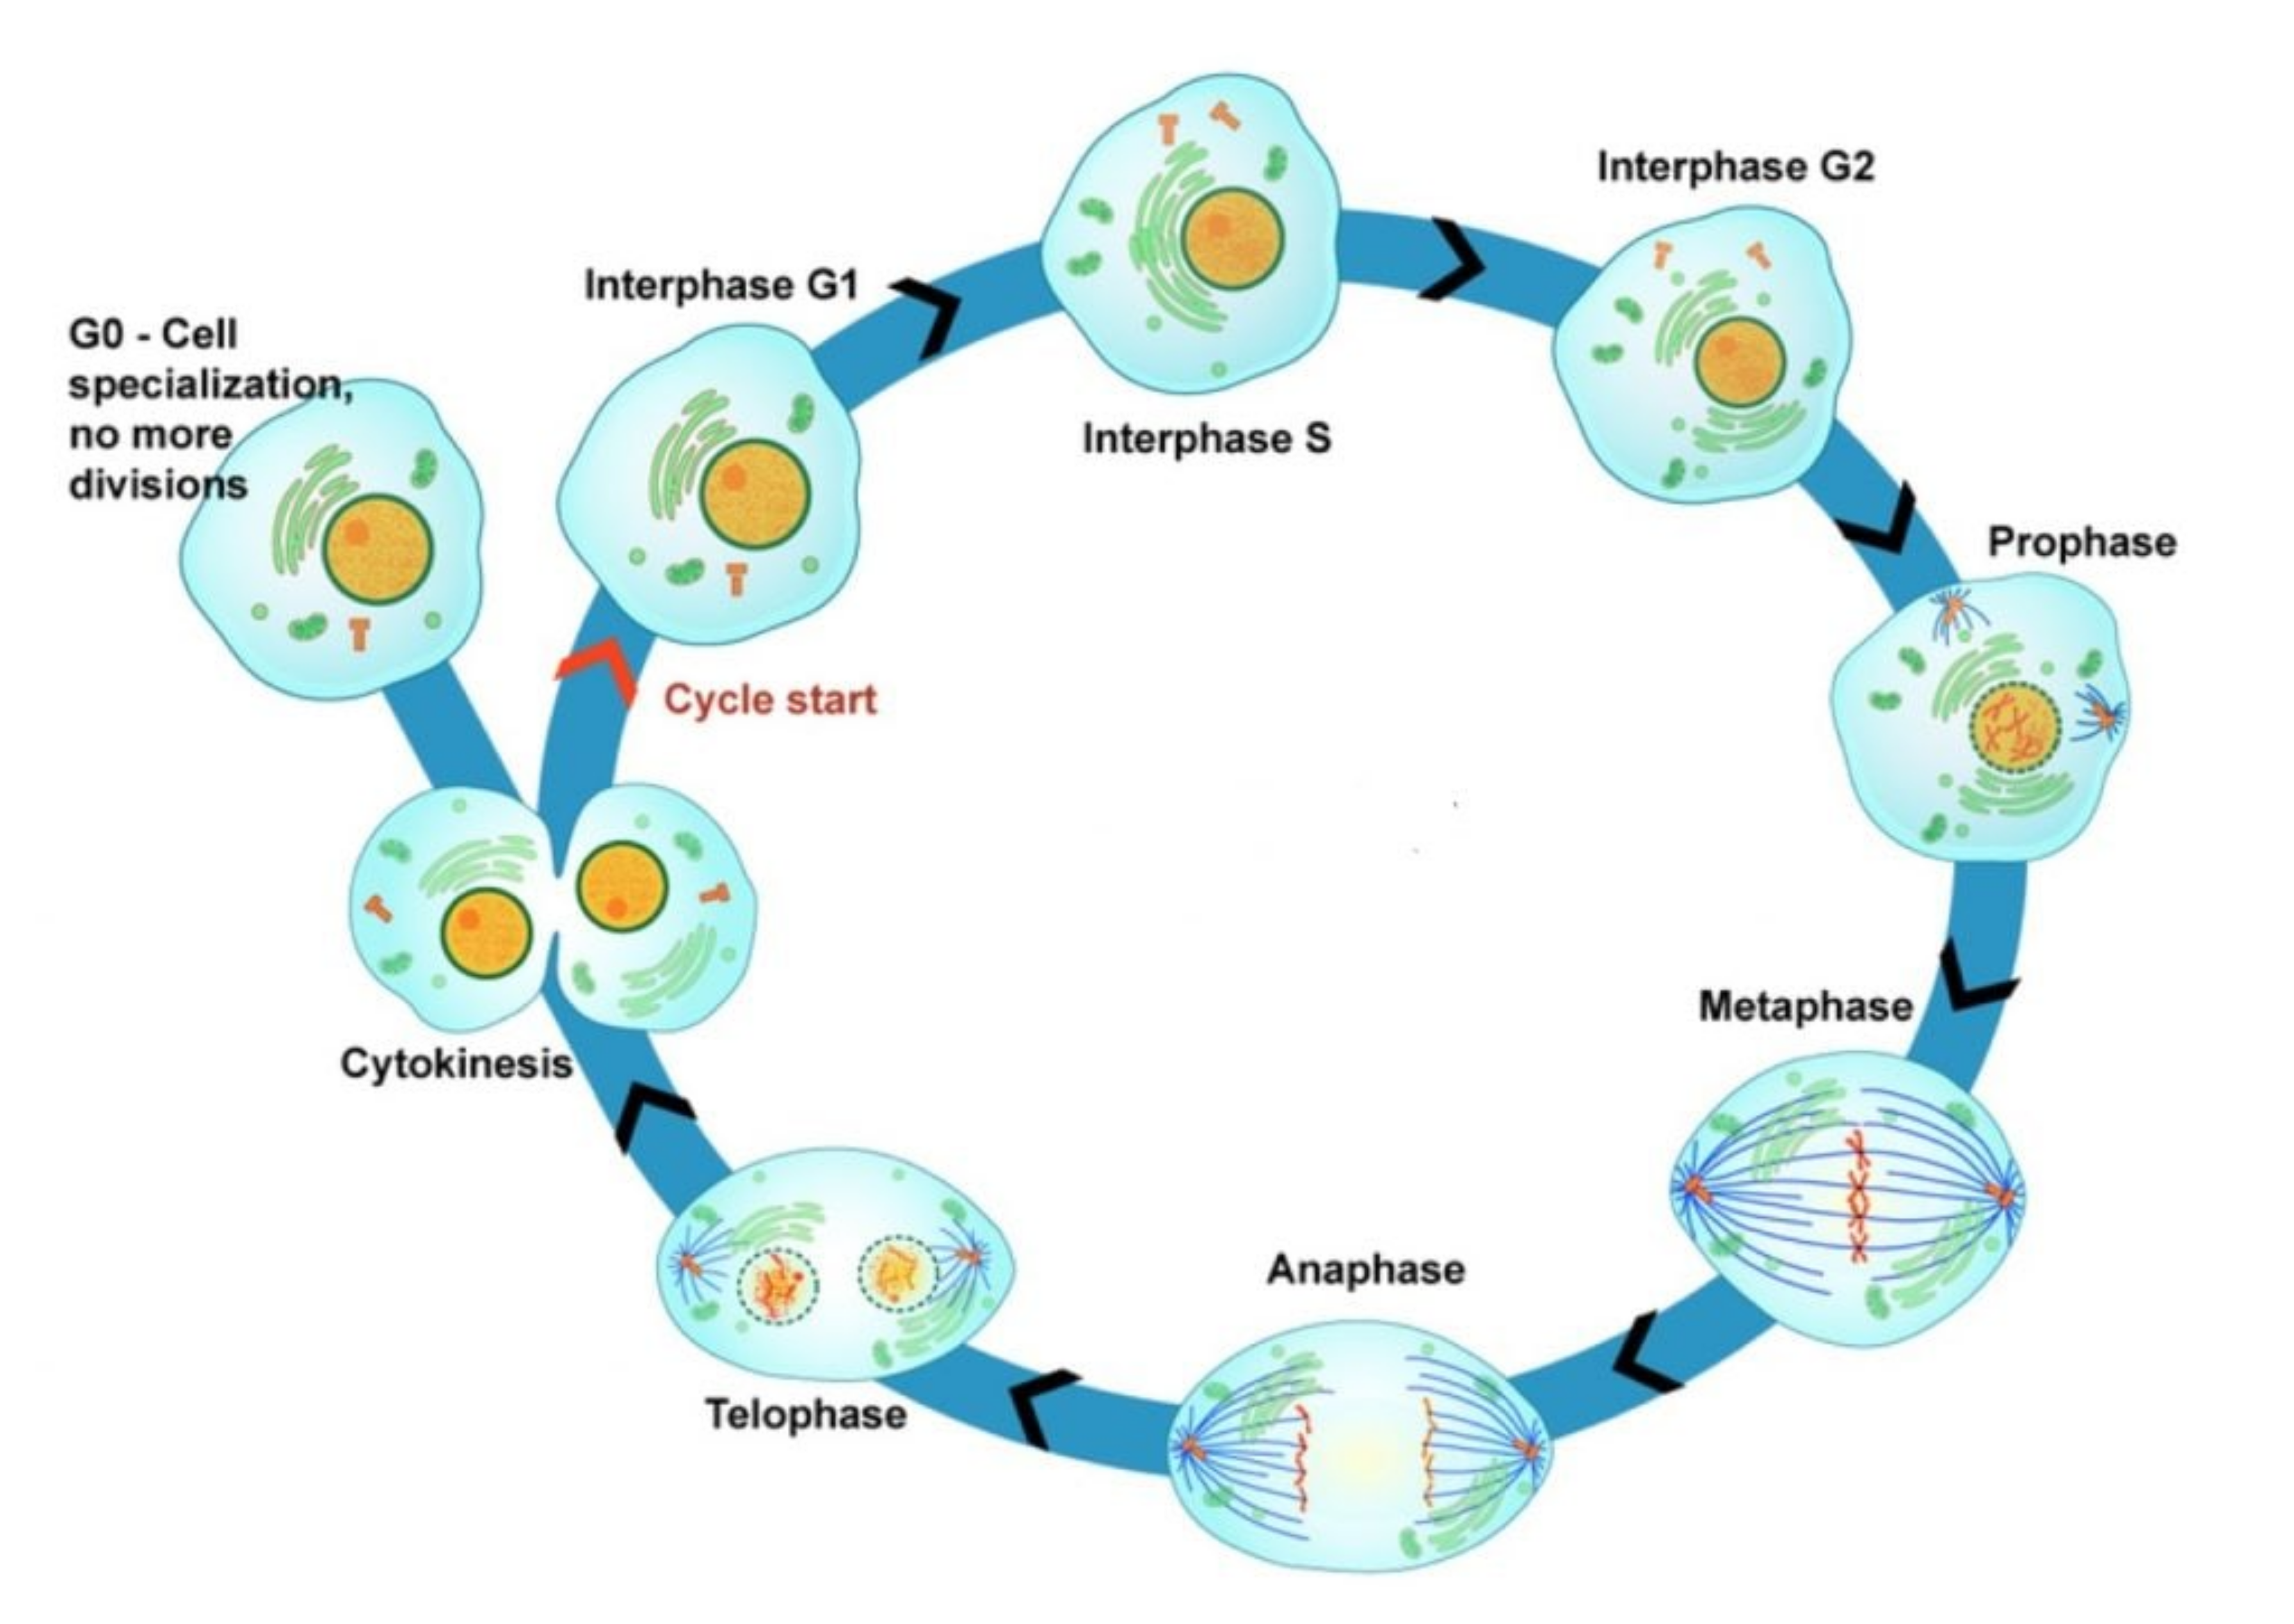
\includegraphics[width=\textwidth]{mitosis.png}
       		\caption{Etapas reproducción celular}
       		\label{fig:repCelular}
       	\end{subfigure}
       	~
       	\begin{subfigure}[b]{0.3\textwidth}
       		\begin{tikzpicture}[]
       		%\draw[] (0,0) arc (0:220:1);
       		\draw[]
       		(0,0) circle (0.875)
       		(0,0) circle (1)
       		(0,0) circle (1.15)
       		;
       		\draw[rotate={70}](0.875,0)--(1.25,0);
       		\draw[rotate={110}](0.875,0)--(1.25,0);
       		\draw[rotate={230}](0.875,0)--(1.25,0);
       		\draw[rotate={300}](0.875,0)--(1.25,0);
       		%\fill[black] (-0.05,0) -- (0.05,0) -- (0,0.1);
       		
       		%PRIMER PAR DE FLECHAs
       		\fill[black,rotate={70}] (0+1.15,0)--(0.025+1.15,0.05) -- (-0.025+1.15,0.05);
       		\fill[black,rotate={70}] (0+1.15,0)--(0.025+1.15,-0.05) -- (-0.025+1.15,-0.05);
       		
       		%Segundo PAR DE FLECHAs
       		\fill[black,rotate={110}] (0+1.15,0)--(0.025+1.15,0.05) -- (-0.025+1.15,0.05);
       		\fill[black,rotate={110}] (0+1.15,0)--(0.025+1.15,-0.05) -- (-0.025+1.15,-0.05);
       		
       		%TERCER PAR DE FLECHAs
       		\fill[black,rotate={230}] (0+1.15,0)--(0.025+1.15,0.05) -- (-0.025+1.15,0.05);
       		\fill[black,rotate={230}] (0+1.15,0)--(0.025+1.15,-0.05) -- (-0.025+1.15,-0.05);
       		
       		%CUERTO PAR DE FLECHAs
       		\fill[black,rotate={300}] (0+1.15,0)--(0.025+1.15,0.05) -- (-0.025+1.15,0.05);
       		\fill[black,rotate={300}] (0+1.15,0)--(0.025+1.15,-0.05) -- (-0.025+1.15,-0.05);
       		
       		%ARRIBA
       		%\fill[black] (0,0)--(0.05,0.1) -- (-0.05,0.1);
       		%DERECHA
       		%\fill[black] (0,0)--(0.1,-0.05) -- (0.1,0.05);
       		%IZQUIERDA
       		%\fill[black] (0,0)--(-0.1,-0.05) -- (-0.1,0.05);
       		%ABAJO
       		%\fill[black] (0,0)--(0.05,-0.1) -- (-0.05,-0.1);
       		
       		\node[] at(1.4,0){$G_1$};
       		\node[] at(-1.4,0){$G_2$};
       		\node[] at(0,1.6){$M$};
       		\node[] at(0,1.3){(mitosis)};
       		\node[] at(0,-1.4){S (Síntesis ADN)};
       		\end{tikzpicture}
       		\caption{Ciclo mitótico de una célula}
       		\label{mititicCycle}
       	\end{subfigure}
       	\caption{Reproducción Celular}
       	\label{repCelularGanz}
       \end{figure}
        	
 \end{frame}

%------------------------------------------------


\subsection{Mecanismos de los efectos de la radiación.}

%------------------------------------------------
\begin{frame}
	
	\begin{figure}[h!]
		\begin{minipage}[t][3.5cm]{\textwidth}
			\begin{center}
				\smartdiagramset{
					%uniform color list=gray!60!black for 3 items,
					back arrow disabled=true,
					additions={
						additional item offset=0.85cm,
						additional item border color=blue,
						%additional arrow color=red,
						%additional arrow tip=stealth,
						%additional arrow line width=1pt,
						%additional arrow style=]-latex’,
					}
				}
				\smartdiagramadd[bubble diagram:horizontal]{Efectos de la radiación,Estoclásticos,No estoclásticos}{%
					below of module2/Determina por dosis Cáncer Mutaciones, below of module3/Predecibles Efectos hematológicos%
				}
			\end{center}
		\end{minipage}
		\caption{}
		\label{efectosRadiacion}
	\end{figure}
\end{frame}

%------------------------------------------------

\begin{frame}
	
	\begin{block}{}
		El resultado final de estas transformaciones químicas en una célula depende de qué moléculas celulares se ven afectadas.\\
	\end{block}

  \begin{block}{}
    
     Con respecto a los efectos estocásticos y no estocásticos observables, las partes más sensibles de la célula se encuentra dentro del núcleo celular, como con los cromosomas.\\	
  \end{block}

  \begin{block}{}
	Los eventos que tienen lugar dentro de los núcleos son cruciales para el bienestar de la célula en su conjunto y pueden transmitirse a la progenie celular en la mitosis.\\
\end{block}

\end{frame}

%------------------------------------------------

\section{Muerte Celular}

%------------------------------------------------

\begin{frame}
   
   
   \begin{block}{}
   	   Cuando la fracción de células supervivientes se representa frente a la dosis de radiación. En todos los casos, los sobrevivientes la fracción disminuye con los aumentos en la dosis absorbida.
   \end{block}


\begin{block}{LET (Linear Energy Transfer/Transferencia lineal de energía)}

    \begin{itemize}
    	\item Alta
    	\item Baja
    \end{itemize}

\end{block}

   
   \begin{block}{}
   	El efecto de la alta radiación LET es mayor que el de baja radiación LET por dosis absorbida.
   \end{block}
   
   	
\end{frame}

%------------------------------------------------

\begin{frame}
   \begin{figure}[h!]
   	\centering
   	\begin{tikzpicture}
      	
   	%\draw (-2,0) -- (2,0);
   	%\filldraw [gray] (0,0) circle (2pt);
   	%CURVA BEZIER CON 3 PUNTOS
   	\draw [blue,thick](0,4.5) .. controls (2,3.75) .. (4.5,0.5);
   	%CURVA ROJA
   	\draw[red,thick](0,4.5)--(1.5,0.5);	
   	\draw[thick]
   	(0,0)--(5,0)
   	(0,0)--(0,5)
   	;
   	\draw[thick]
   	%marca200
   	(0.8,0)--(0.8,0.25)
   	%marca400
   	(1.7,0)--(1.7,0.25)
   	%marca600
   	(2.5,0)--(2.5,0.25)
   	%marca800
   	(3.3,0)--(3.3,0.25)
   	%marca1000
   	(4.2,0)--(4.2,0.25)
   	%marca1200
   	(5,0)--(5,0.25)
   	;
   	\draw[dashed,gray]
   	(0,1.5)--(5,1.5)
   	(0,3)--(5,3)
   	(0,4.5)--(5,4.5)
   	;
   	%\draw (-2,2) .. controls (-1,0) and (1,0) .. (2,2);
   	
   	\node[rotate={90}] at(0.8,-0.5){200};
   	\node[rotate={90}] at(1.7,-0.5){400};
   	\node[rotate={90}] at(2.5,-0.5){600};
   	\node[rotate={90}] at(3.3,-0.5){800};
   	\node[rotate={90}] at(4.2,-0.5){1000};
   	\node[rotate={90}] at(5,-0.5){1200};
   	
   	\node[] at(2.5,-1.25){Radiaciones};
   	
   	\node[] at(-0.5,0){$10^{-3}$};
   	\node[] at(-0.5,1.5){$10^{-2}$};
   	\node[] at(-0.5,3){$10^{-1}$};
   	\node[] at(-0.5,4.5){1};
   	
   	\node[rotate={90}] at(-1.25,2.25){Fracción superviviente};
   	
   	\draw[gray] (3,3.2) rectangle (7.5,4.6);
   	\draw[red,thick](3.25,4.25)--(3.625,4.25);
   	\draw[blue,thick](3.25,3.5)--(3.625,3.5);
   	\node[] at(5.5,4.25){Radiación LET Alta};
   	\node[] at(5.5,3.5){Radiación LET Baja};
   	
   	\end{tikzpicture}
   	\caption{Curvas de supervivencia de células expuestas a dosis agudas de radiación}
   \end{figure}
   	
\end{frame}

%------------------------------------------------
 
\begin{frame}
   
   \begin{block}{La muerte celular}
     Es un proceso no estocástico, explica los efectos que se observan después de la exposición aguda de individuos a la radiación. Estos efectos, dependerán de cuántas células mueran y de la función normal o el propósito de Células.\\	
   \end{block}
   \begin{center}
   	\centering
   	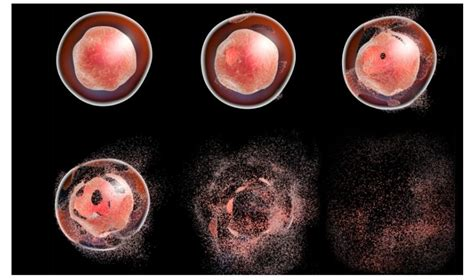
\includegraphics[width=0.5\textwidth]{muerteCelular}
   \end{center}
   
\end{frame} 

%------------------------------------------------

\section{Cáncer}

%------------------------------------------------

\begin{frame}
	\frametitle{Cáncer en México}
	\begin{table}[h!]	
		\centering
		\begin{tabular}{||c|c|c|c|c||}
			\hline
			\textbf{Tipo de Cáncer }      & \textbf{0 a 17} & \textbf{18 a 29} & \textbf{18 a 29} & \textbf{< 60} \\ \hline\hline
			Órganos hematopoyéticos                & 2.41 & 2.48 & 3.96 &   \\ 
			Huesos                                 & 0.33 &      &      &     \\ 
			Tejidos mesoteliales                   & 0.17 &      &      &     \\ 
			Testículo u ovario                     &      & 1.35 & 8.52 & 85*    \\ 
			Mama                                   &      &      & 7.61 & 25.23 \\ 
			Órganos respiratorios                  &      &      & 3.65 & 50.39 \\ 
			Órganos digestivos                     &      & 1.15 & 15.68& 152.56     \\ 
			Tejido linfático                       & 0.23 & 0.76 &      & \\ 
			Encéfalo y sistema nervioso            & 0.71 & 0.57 &      &  \\ \hline 
		\end{tabular}
		\caption{Tasa de mortalidad población por edades 2016 por cada 100 00 habitantes}
	\end{table}
	
\end{frame}

%------------------------------------------------

\begin{frame}
	
	\frametitle{Carcinógenos}
	
   Hay químicos, llamados carcinógenos, que son conocidos por producir cáncer Se cree que más del 90 $\%$ de todos los cánceres humanos son resultado de carcinógenos en el medio ambiente, la mayoría de los cuales se producen naturalmente.\\
   
   \begin{center}
   	\centering
   	
\includegraphics[width=0.3\textwidth]{peligroBiologico}
   \end{center}
   
\end{frame}
   
%------------------------------------------------
   
\begin{frame}
	   %Las causas precisas del cáncer no se conocen a partir de este escrito. 
	   
	   \begin{block}{}
	   La creciente inducción del cáncer es un proceso de dos etapas.\\
	   \end{block}
	   
	   \begin{block}{Primero}
	     Se produce una lesión (es decir, alguna lesión u otro efecto perjudicial) en el ADN en una o varias células. Las células afectadas se transforman así en células potencialmente cancerosas, a punto de sufrir una división incontrolada. 
	   \end{block}
	   
	   \begin{block}{Segundo}
	   	Algunas personas aún no identificadas, inmunológicas, les impiden hacerlo u otro agente protector. Tales agentes son probablemente características heredadas de cada individuo.\\	
	   \end{block}
	    
\end{frame}

%------------------------------------------------

\begin{frame}
	Durante la segunda etapa de herencia, el mecanismo de protección falla por alguna razón y permite, las células iniciadas se multiplican sin restricciones. La etapa de herencia puede ser provocada por factores tan diversos como las infecciones virales, irritantes químicos, falla del sistema inmunológico o fisiológica cambios en el cuerpo que ocurren naturalmente con el envejecimiento.\\
	
	\begin{block}{}
		La teoría del cáncer de dos estados explica el hecho de que hay un período latente de varios años entre el momento de la irradiación y la aparición de muchos tipos de cánceres, durante los cuales la probabilidad de que ocurra un cáncer es esencialmente cero.\\
	\end{block}

\end{frame}

%------------------------------------------------

\begin{frame}

 	\frametitle{Herencia}
   
 \begin{block}{}
 	    Puede haber segmentos de la población que es especialmente susceptible o resistente al cáncer inducido por radiación, se desconoce actualmente el agente responsable de ésto pero se especula sobre información genética en particular.
 \end{block}   
   
   \begin{block}{}
   	La célula o las células se desencadenaron en malignidad durante la etapa de herencia generalmente no son las mismas células iniciadas durante la irradiación.
   \end{block} 
    
\end{frame}
   
%------------------------------------------------

\subsection{Efectos genéticos}

%\subsection{Subsection Example} % A subsection can be created just before a set of slides with a common theme to further break down your presentation into chunks

%------------------------------------------------

\begin{frame}
	\frametitle{ADN y mutaciones}
  
  \begin{block}{}
  	  Si la radiación logra alterar una molécula de ADN en un cromosoma, el resultado puede ser una mutación 
  \end{block}

  
  %Si la mutación ocurre en una célula somática de un desarrollo completo individual, no se puede observar ningún efecto macroscópico a menos que se encuentren muchas células igualmente, involucrados Esto se debe a que el ADN determina la estructura de las proteínas.
  %fabricado por la célula, y una mutación por lo tanto interfiere con la producción de Las proteínas necesarias para el correcto funcionamiento celular. 
  
  
  \begin{block}{}
  	 Las mutaciones son generalmente dañino para las células y la progenie de una célula mutante, no en sí para la célula madre
  \end{block}
 
  \begin{block}{célula germinal}
  	la célula afectada es
  	generalmente incapaz de ser fertilizado. Si el gameto mutante es exitoso fertilizado y el cigoto se convierte en una descendencia viva, luego se lleva la mutación en la progenie. 
  \end{block}
  
  %\begin{block}{}
  %	Por esta razón, la exposición a la radiación de las gónadas es especial.\\	
  %\end{block}
  
\end{frame}
  
  %------------------------------------------------


\begin{frame}
	\frametitle{Mutaciones}
	
   Las mutaciones ocurren espontáneamente en la población humana de causas de origen desconocido, aproximadamente 10 $\%$ de todos los recién nacidos sufren directamente de un trastorno o mal funcionamiento de origen genético o portar tales defectos, que se expresan más tarde en la vida o en su progenie.\\
   
   \begin{block}{Efecto de la radiación en los humanos}
   	Con los estudios de las víctimas y sobrevivientes de los bombardeos atómicos de la Segunda Guerra Mundial en Japón; y en numerosos experimentos con animales de laboratorio. La situación actual de estos estudios se puede resumir de la siguiente manera:\\	
   \end{block}
   
   
\end{frame}

%------------------------------------------------

\begin{frame}
    
    \begin{enumerate}
    	\item Existe información sobre los efectos de grandes, agudos (a corto plazo)	dosis de radiación, superiores a 1 0 a 20 rems.
    	\item Debido a que los efectos son tan raros, si es que existen, solo hay datos limitados
    	mostrando efectos positivos de:	
    	\begin{enumerate}
    		\item Dosis agudas de hasta 1 0 o 20 rems y no repetidas;
    		\item Dosis agudas de algunos rems y repetidas ocasionalmente; y
    		\item Dosis crónicas (que continúan durante mucho tiempo) del orden de mili rems por día.
    	\end{enumerate}	
    \end{enumerate}	
\end{frame}

%------------------------------------------------

%%%\subsection{Grandes dosis agudas: efectos tempranos}


\begin{frame}
	Los efectos de las dosis agudas, se distinguen entre los efectos tempranos
	
	\begin{block}{Efectos Tempranos}
		Son evidentes dentro de los 60 días de la exposición
	\end{block}

    \begin{block}{Efectos tardíos}
    	Después de 60 días
    \end{block}
  
  Los primeros efectos son generalmente de naturaleza no estocástica; Los efectos tardíos surgen de los procesos estocásticos y no estocásticos. 

\end{frame}

%------------------------------------------------

\begin{frame}
	
	\begin{table}[h!]
		\centering
		\begin{tabular}{||m{1cm}|m{20em}||}
			\hline
			\multicolumn{2}{|c|}{Probables primeros efectos de la radiación aguda de el cuerpodosis*t} \\
			\hline	\hline
			(rems)                                                            & Probable efecto observado                                                                                                                                                          \\ \hline
			5 a 75                                                                       & Aberraciones cromosómicas y depresión temporal de los niveles de glóbulos blancos en algunos individuos. No hay otros efectos observables.                                                                                                                                                                                                                                                                                                                          \\ \hline
			75 a 200                                                                     & Vómitos en 5 a 50\% de las personas expuestas en pocas horas, con fatiga y pérdida de apetito, cambios moderados de sangre. Recuperación en pocas semanas para la mayoría de los síntomas.                                                                                                                                                                                                                                                                          \\ \hline
		\end{tabular}
		\caption{Probales primeros efectos}
	\end{table}
	
\end{frame}

%------------------------------------------------

\begin{frame}
	
	\begin{table}[h!]
		\centering
		\begin{tabular}{||m{1cm}|m{20em}||}
			\hline
			\multicolumn{2}{|c|}{Probables primeros efectos de la radiación aguda de el cuerpodosis*t} \\
			\hline	\hline
			(rems)                                                            & Probable efecto observado                                                                                                                                                          			\\ \hline
			200 a 600                                                                    & Para dosis de 300 rems o más, todas las personas expuestas exhibirán vómitos dentro de las 2 horas. Cambios sanguíneos severos, con hemorragia y mayor susceptibilidad a la infección, particularmente a dosis más altas. Pérdida de cabello después de 2 semanas para dosis de más de 300 rems. Recuperación de 1 mes a un año para la mayoría de las personas en el extremo inferior del rango de dosis; sólo el 20\% sobrevive en el extremo superior del rango. \\ \hline
		\end{tabular}
		\caption{Probales primeros efectos}
	\end{table}
	
\end{frame}

%------------------------------------------------

\begin{frame}
	
	\begin{table}[h!]
		\centering
		\begin{tabular}{||m{1cm}|m{20em}||}
			\hline
			\multicolumn{2}{|c|}{Probables primeros efectos de la radiación aguda de el cuerpodosis*t} \\
			\hline	\hline
			(rems)                                                            & Probable efecto observado                              	\\ \hline
			600 a 1, 000                                                                 & Vómitos en 1 hora. Cambios sanguíneos severos, hemorragia, infección y pérdida de cabello. Del 80\% al 1 00\% de las personas expuestas sucumbirán en 2 meses; los que sobrevivan serán convalecientes durante un largo período.                                                                                                                                                                                                                                    \\ \hline
		\end{tabular}
		\caption{Probales primeros efectos}
	\end{table}
	
\end{frame}

%------------------------------------------------

\begin{frame}
	
	\begin{block}{}
			No se aprecian efectos nocivos graves para dosis de menos de aproximadamente 75 rems. A dosis mayores de 75 rems, se dice que el individuo expuesto sufre de síndrome de radiación aguda.
	\end{block}

\end{frame}

%------------------------------------------------

\begin{frame}
	Los efectos se pueden representar en las siguientes cuatro clases generales clínicamente observables:
	
	\begin{enumerate}
		\item  Trastornos de un solo gen que surgen de una mutación en un punto específico de un cromosoma.
		\item Trastornos multifactoriales debido a mutaciones de puntos múltiples. (El efecto de la radiación
		en producir tales defectos es difícil de evaluar.)
		\item Aberraciones cromosómicas causadas por la presencia de demasiado o muy poco
		material genético en las células (síndrome de Down, por ejemplo).
		\item Abortos espontáneos.	
	\end{enumerate}
	
\end{frame}

%------------------------------------------------

%%%%\subsection{Efectos degenerativos} 

\begin{frame}
	
	\begin{block}{Efectos degenerativos}
		La radiación provoca un aumento en la incidencia de condiciones degenerativas en varios órganos del cuerpo debido a la falla de los tejidos expuestos para regenerarse adecuadamente.\\
	\end{block}

    \begin{block}{Acotamiento de la vida}
    	El efecto general de la exposición a la radiación puede verse en su influencia en la vida útil de las personas expuestas. Es de esperar, aunque solo sea sobre la base de los otros efectos a largo plazo.\\
    \end{block}

   \begin{block}{Dosis bajas crónicas}
	Las dosis de unos pocos milirems por día, que se acumulan hasta unos pocos rems por año, son motivo de gran preocupación en el desarrollo de la energía nuclear.\\
  \end{block}

\end{frame}

%------------------------------------------------

\section{La radiación LET alta y baja induce de manera diferencial la normalidad
	Señales de daño tisular}

%%%%\subsection{Propósito}


\begin{frame}
	\frametitle{Descripción}
	 La radioterapia que utiliza radiación de alta transferencia de energía lineal (LET) tiene como objetivo eliminar las células tumorales al mismo tiempo que minimiza la dosis (biológicamente efectiva) a los tejidos normales.
	para prevenir la toxicidad. Está bien establecido que una alta radiación LET da como resultado una célula más baja.
	supervivencia por dosis absorbida que la radiación LET baja. Sin embargo, si varios mecanismos
	que participan en el desarrollo de daño tisular normal puede ser regulado de manera diferencial es
	no se conoce. Por lo tanto, el objetivo de este estudio era investigar si dos acciones relacionadas con
	a la toxicidad tisular normal, la apoptosis inducida por p53 y la expresión del gen profibrótico
	PAI-1 (inhibidor del activador del plasminógeno 1), son inducidos diferencialmente por alto y bajo LET
	radiación.
\end{frame}


%%%%\subsection{Métodos y materiales}

\begin{frame}
	\frametitle{Resultados}
	Las células fueron irradiadas con iones de carbono LET alto o fotones LET bajo.
	Se realizaron ensayos de supervivencia celular, la expresión profibrótica de PAI-1 fue monitoreada por análisis cuantitativos.
	la reacción en cadena de la polimerasa, y la apoptosis fue ensayada por la tinción de la anexión V. Activación de p53
	por fosforilación en la serina 315 y la serina 37 fue monitoreada por Western blotting. Transfect--
	para el ensayo de los plásmidos que expresan p53 mutados en las serinas 315 y 37 se utilizaron para el ensayo del requisito
	de estos residuos para la apoptosis y la expresión de PAI-1.
	
\end{frame}


%%%%\subsection{Resultados}

\begin{frame}
	\frametitle{Conclusión}
	Como era de esperar, la supervivencia celular fue menor y la inducción de la apoptosis fue mayor en alta -LET
	células irradiadas. Interesantemente, la inducción del gen PAI-1 profibrótico fue similar con un alto nivel de glucosa y
	baja radiación LET. De acuerdo con este hallazgo, la fosforilación de la p53 en la serina 315 implica
	en la expresión de PAI-1 fue similar con radiación LET alta y baja, mientras que la fosforilación de
	p53 en la serina 37, involucrada en la inducción de apoptosis, fue mucho más alta después de una alta irradiación de LET.
	
\end{frame}

%%%%\subsection{Conclusiones}


\begin{frame}
	Nuestros resultados indican que los diversos mecanismos que intervienen en el desarrollo del
	El daño tisular normal puede verse afectado diferencialmente por la radiación LET alta y baja. Esto puede
	tienen consecuencias para el desarrollo y la manifestación de daño tisular normal.
\end{frame}

\section{Estadísticas del daño del cáncer en México}

\begin{frame}
	
	\begin{enumerate}
		\item Durante el lapso de 2011 a 2016, dos de cada 100 000 habitantes de 0 a 17 años
		fallecen anualmente por un tumor en órganos hematopoyéticos (conformado
		entre otros, por la leucemia). Entre los jóvenes de 18 a 29 años, mueren tres de
		cada 100 000 hombres contra dos de cada 100 000 mujeres por esta causa
		\item Tres de cada 10 muertes por cáncer en la población de 30 a 59 años, son
		consecuencia del cáncer en órganos digestivos. Para la población de 60 y más
		años, de 2011 a 2016, cuatro de cada 10 defunciones por cáncer en mujeres se
		deben a tumor en órganos digestivos, contra tres de cada 10 en varones, por la
		misma causa
		\item Respecto al cáncer de mama, en 2016 se observan 16 defunciones por cada
		100 000 mujeres de 20 años y más
	\end{enumerate}
	
\end{frame}

\begin{frame}	
	
	\begin{block}{}
		El cáncer es la principal causa de muerte a nivel mundial; en 2015 se calcula que provocó 8.8
		millones de defunciones, y se identifican cinco tipos de cáncer responsables del mayor número de
		fallecimientos: cáncer pulmonar (1,69 millones de muertes), cáncer hepático (788 000 defunciones),
		cáncer colorrectal (774 000 muertes), cáncer gástrico (754 000 defunciones) y de mama (571 000
		muertes) (Organización Mundial de la Salud [OMS], 2017).
	\end{block}
\end{frame}


%\begin{frame}
%\frametitle{Theorem}
%\begin{theorem}[Mass--energy equivalence]
%$E = mc^2$
%\end{theorem}
%\end{frame}

%------------------------------------------------

%\begin{frame}[fragile] % Need to use the fragile option when verbatim is used in the slide
%\frametitle{Verbatim}
%\begin{example}[Theorem Slide Code]
%\begin{verbatim}
%\begin{frame}
%\frametitle{Theorem}
%\begin{theorem}[Mass--energy equivalence]
%$E = mc^2$
%\end{theorem}
%\end{frame}\end{verbatim}
%\end{example}
%\end{frame}

%------------------------------------------------
%\begin{frame}
%\begin{frame}[fragile] % Need to use the fragile option when verbatim is used in the slide
%\frametitle{Citation}
%An example of the \verb|\cite| command to cite within the presentation:\\~

%This statement requires citation \cite{p1}.

%\end{frame}

%------------------------------------------------

\begin{frame}
\frametitle{Referencias}

\footnotesize{
\begin{thebibliography}{99} % Beamer does not support BibTeX so references must be inserted manually as below
\bibitem[Lamarsh2001]{p1} Lamarsh, John R and Baratta, Anthony J (2012)
\newblock Introduction to Nuclear Engineering
\newblock \emph{Third}. 

\bibitem[InstitutoNacionalDeEstadisticayGeografia2018]{p2} INEGI (2018)
\newblock cancer2018
\newblock \emph{4 Febrero}.

\bibitem[Niemantsverdriet2012]{p3} Niemantsverdriet (2012)
\newblock High and low LET radiation differentially induce normal tissue damage signals
\newblock \emph{2012}.
\end{thebibliography}
}
\end{frame}

%------------------------------------------------

\begin{frame}
\Huge{\centerline{¡Gracias por su atención :D !}}
\end{frame}

%----------------------------------------------------------------------------------------

\end{document} 